\section{Version control using Helix Core\textsuperscript{\texttrademark}}
In this section, a very basic 2D game is created with the game engine Godot. The development process is version 
controlled using the Helix Core application to demonstrate the major steps and show the differences compared to 
traditional SW development workflow.
\begin{itemize}
    \item centralized version control system: files are maintained on centralized server
    \item files are stored in depos: typically 1 depo per project
    \item workspace: mapping of relevant files between local machine and server
\end{itemize}

\subsection{Setup Helix Core}
The setup of Helix Core follows the instructions from the 
\href{https://help.perforce.com/helix-core/quickstart/Content/quickstart/admin-install-linux.html}{\color{blue}{Helix Core Server Administrator Guide}}
relevant for Linux (Ubuntu) systems. The following commands were issued for setting up the version control application, as 
can be found in the aformentioned documentation.
\begin{enumerate}
    \item Download perforce public key
    \begin{verbatim}
        $ wget https://package.perforce.com/perforce.pubkey
    \end{verbatim}
    \item Obtain the fingerprint of the public key and verify
    \begin{verbatim}
        $ gpg -n --import --import-options import-show perforce.pubkey
        $ gpg -n --import --import-options import-show perforce.pubkey | 
        grep -q "E58131C0AEA7B082C6DC4C937123CB760FF18869" && echo "true"
    \end{verbatim}
    \item Add the public key to your keyring
    \begin{verbatim}
        $ wget -qO - https://package.perforce.com/perforce.pubkey | 
        sudo apt-key add -
    \end{verbatim}
    \item Create a new file for the Perforce repository
    \begin{verbatim}
        $ sudo nano /etc/apt/sources.list.d/perforce.list
    \end{verbatim}
    \item In the new file, input the following line
    \begin{verbatim}
        deb http://package.perforce.com/apt/ubuntu focal release
    \end{verbatim}
    \item Update machine and install Helix Core
    \begin{verbatim}
        $ sudo apt-get update
        $ sudo apt-get install helix-p4d
    \end{verbatim}
    \item Run configure file
    \begin{verbatim}
        $ sudo /opt/perforce/sbin/configure-helix-p4d.sh
    \end{verbatim}
    \item Download visual interface (p4v) from 
    \href{https://www.perforce.com/downloads/helix-visual-client-p4v}{\color{blue} Download Page}.
    P4v is the client application commnicating with the server. Server in this case is created on local machine.
    \item Additional config steps
    \begin{verbatim}
        $ export P4PORT=ssl:1666
        $ export P4USER=super
        # add the following line to ~/.bashrc
        export PATH=${PATH}:~/perforce/p4v-2023.3.2495381/bin
    \end{verbatim}
    \item Login and start p4v
    \begin{verbatim}
        $ p4 login
        $ p4v # launches GUI
    \end{verbatim}
\end{enumerate}
Having done the above steps, the GUI can be launched bringing up the screen below. The location of the server (where
all shared files/projects are stored) \colorbox{blue!30}{/opt/perforce/servers/master/root} 
As the server is also created on local machine. This folder is used to create the mapping between server and other 
client machines and workspaces.
\begin{figure}[H]
    \centering
    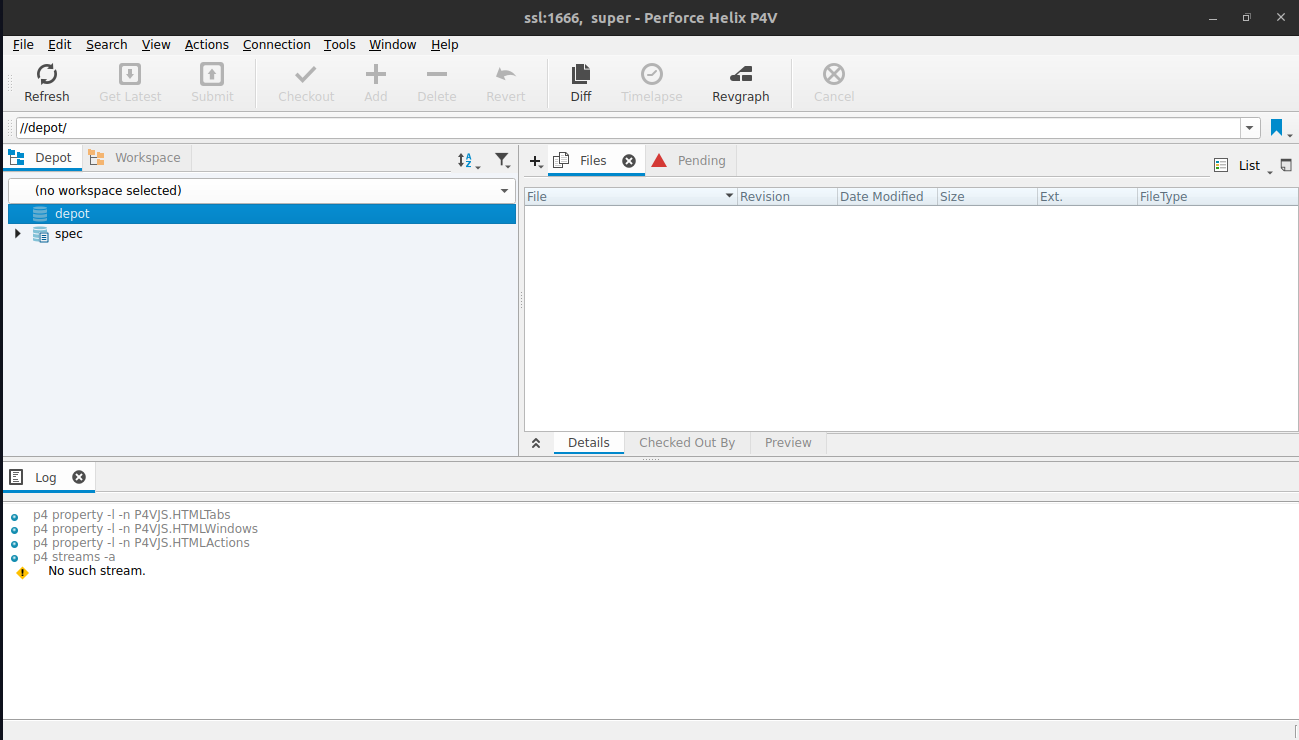
\includegraphics[width=\textwidth]{p4vlogin20231029.png}
      \caption{p4v login}
      \label{fig:p4v login}
\end{figure}

\subsection{Setup Godot}
Setting up Godot game engine is relatively easy compared to other game engines like Unity\textsuperscript{\texttrademark}
or Unreal Engine\textsuperscript{\texttrademark}. Godot is lightweight and there are basically two options to get hold
of the application:
\begin{itemize}
    \item Download pre-build application specific to host machine OS and programming language (GDScript or .Net)
    \href{https://godotengine.org/download/linux/}{\color{blue}Download page}
    \item Build from source following instructions 
    \href{https://docs.godotengine.org/en/stable/contributing/development/compiling/index.html}{\color{blue}Build from source}.
\end{itemize}
For the purpose of this paper the first approach was followed by downloading the Godot 4.1.2 stable version for Linux.
After downloading and unpacking, Godot is ready to use:
\begin{figure}[H]
    \centering
    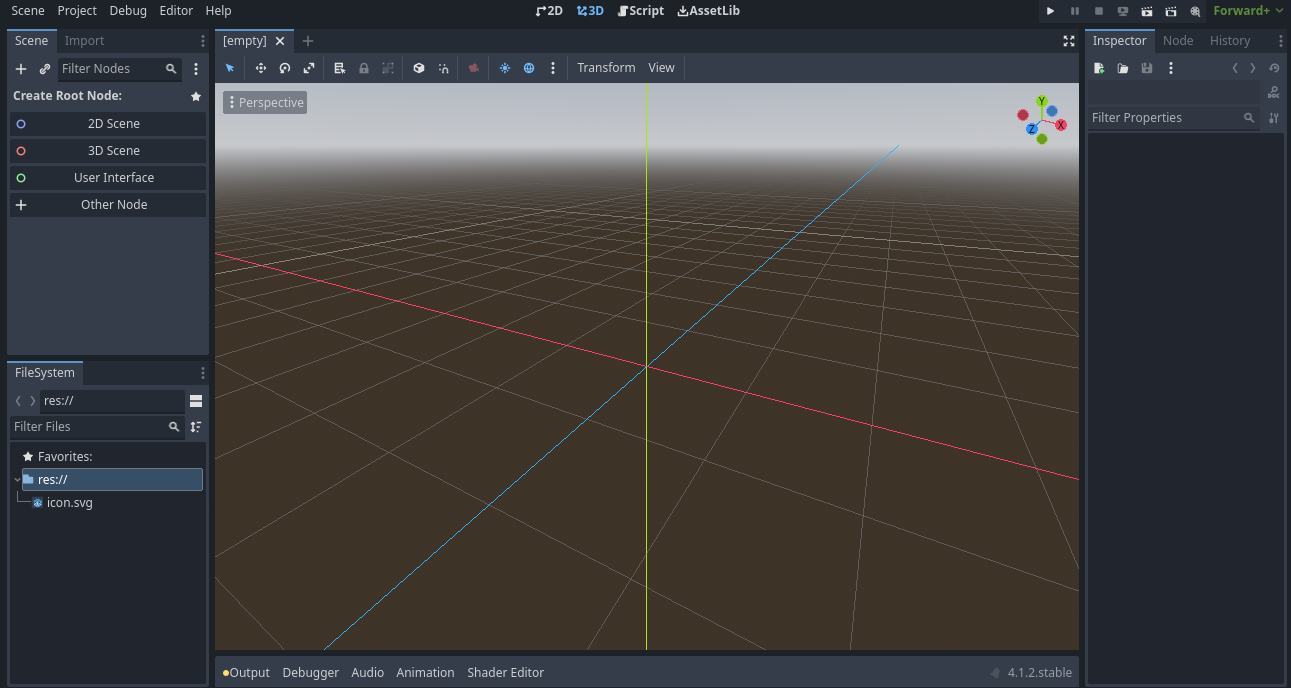
\includegraphics[width=\textwidth]{godotopen.png}
      \caption{godot}
      \label{fig:godot}
\end{figure}

\subsection{Development and version control}
\begin{itemize}
    \item 2D game using 
    \href{https://docs.godotengine.org/en/stable/getting_started/first_2d_game/index.html}{\color{blue}Godot 2D game instructions}
    \item create empty godot project
    \item setup workspace for version control with perforce and initial commit
    \item follow development steps with version control
\end{itemize}
